Gyrotron has many applications spanning across a variety of fields due to its capability of generating high power at high frequencies.
Some of these fields include spectroscopy, plasma heating and diagnosis, defence that indicate applicability of gyrotrons.

\section{Defence}

National security is always a top priority for all countries and this leads to development of cutting edge instruments and devices that can help detect all kinds of threats, from a unknown drone to space junk near space stations and act accordingly, to protect their citizens and interests.

\subsection{Military}

Raytheon of the U.S. Army used gyrotrons, gyro-amplifiers in a system they developed, called the Active Denial System (ADS). The ADS system ( see figure \ref{fig:ads} ) is a non-lethal, anti-personnel weapon that uses the directed energy of the gyrotron. The gyrotron used works at 95GHz with an effective power density of $ 2W/m^2 $ covering 1km radius. This device generates waves that penetrates the skin causing a spike in water's temperature thus heating the upper layer of the skin upto 60 degrees celsius causing a second degree burn and inflicting serious pain.

\begin{figure}[H]
\centering
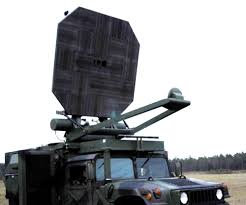
\includegraphics{images/ads}
\caption{Active Denial System, U.S.Army.}
\label{fig:ads}
\end{figure}

\subsection{Radar}

Current radar technologies are based on millimetre wave radars that can fetch high location resolution of tracked objects. Using gyro-sources, primarily the gyro-amplifier gyro-TWT and gyro-klystrons, the effective range of these radars has risen upto several hundred kilometres, which combined with high resolution imaging, gives best results. Russia and U.S.A are using gyro-klystrons based antennas, providing output power in the range of 0.1-0.5 MW.

\section{Scientific Research}

Science has had a need for high power and high frequency devices from the past two centuries and the gyrotrons have shown some good prospects and development in some particular fields. Here, gyrotrons are used as gyrotron oscillators.

\subsection{Nuclear Fission and Plasma}
Nuclear fission and plasma research have extensively focussed on developing gyrotrons which have played a huge role in the progress of the field. ITER (International Thermonuclear Experimental Reactor). The ITER required a highly efficient device capable of generating high output power and long pulse of generated radiation to carry out a controlled nuclear fusion. The ITER uses gyrotron at 170GHz generating output power of 1-2 MW.

\subsection{Material Science}
The radiations generated by gyrotrons are used by a technique called Electron Spin Resonance (ESR). Using this technique, the microstructures of various materials are investigated, studied and tested with the help of tetrahertz radiation. The tetrahertz radiation is also used along with Nuclear Magnetic Resonance (NMR). This NMR spectroscopy is used to study materials such as polymers and in bio-molecular analysis of protein and peptide structures that use low-power gyrotrons such as gyro-BWO to provide tetrahertz radiation.


